\subsubsection{Heat Equation}

The heat equation describes the heat distribution in a given region over time. It can be represented as a system of equations as follows:

\begin{equation*}
\begin{cases}
\partial_t u - \partial_{xx} u = f(t, x) & \text{in } J \times G, \\
u = 0 & \text{on } J \times \partial G, \\
u(0, \cdot) = u_0 & \text{in } G,
\end{cases}
\end{equation*}

Where:
\begin{itemize}
\item The equation $u(0, \cdot) = u_0$ in $G$ represents the \textcolor{blue}{initial condition}.
\item The equation $u = 0$ on $J \times \partial G$ represents the \textcolor{blue}{boundary condition}. Here, it is of Dirichlet type and homogeneous.
\end{itemize}

Such partial differential equations are known as initial-boundary value problems.

\subsubsection{Discretization of the PDE}

To solve the heat equation numerically, we discretize the computational domain $J \times G$ using a \textbf{discrete grid}. The grid is defined as follows:

\begin{equation*}
\{(t_m, x_i)\}, \quad i = 0, \ldots, N+1, \quad m = 0, \ldots, M,
\end{equation*}

where $x_i$ are the \textcolor{blue}{spatial grid points} with a \textcolor{blue}{spacing (or space step size)} of $h$, and $t_m$ are the \textcolor{blue}{time levels} with a \textcolor{blue}{time step size} of $k$.

\medskip

The spatial grid points $x_i$ are determined by the interval $G = (a, b)$ and the number of grid points $N$ as $x_i = a + ih$, where $h = \frac{b-a}{N+1}$. 

The time levels $t_m$ are determined by the interval $J = (0, T)$ and the number of time steps $M$ as $t_m = mk$, where $k = \frac{T}{M}$.

\medskip

Next, we represent the exact solution $u(t, x)$ by its values on the grid:

\begin{equation*}
u(t, x) \rightarrow \{u_{m,i} = u(t_m, x_i)\}, \quad i = 0, \ldots, N+1, \quad m = 0, \ldots, M.
\end{equation*}

\textcolor{blue}{The goal is to approximate the values $\{u^{m}_{i}\}$}. Values of the solution between grid points are then found \textbf{using some interpolation method}.

\subsubsection{The Finite Difference Method (FDM)}

The Finite Difference Method (FDM) is a commonly used numerical method for solving partial differential equations. It approximates the derivatives of a function using only its values on the grid. Let's start by defining the difference quotients, also known as finite differences.

\textbf{Difference Quotients (= Finite Differences)}

Consider a function $g(x)$ of one variable. Assume that $g \in C^2$. Using Taylor's formula, we have:

\begin{equation*}
g' (x) = \frac{g(x + h) - g(x)}{h} - \frac{h}{2} g''(\xi), \quad \xi \in [x, x + h].
\end{equation*}

If $g_i = g(x_i)$ are the values of $g$ on the grid $\{x_i\}$, we obtain:

\begin{equation*}
g' (x_i) = \frac{g_{i+1} - g_i}{h} + O(h) =: {(\delta^{+}_{x} g)}_i + O(h).
\end{equation*}

Similarly, for $g \in C^4$:

\begin{equation*}
g'' (x_i) = \frac{g_{i+1} - 2g_i + g_{i-1}}{h^2} + O(h^2) =: {(\delta_{xx}g)}_i + O(h^2).
\end{equation*}

\subsubsubsection{FD Scheme}

In the Finite Difference Method (FDM), we use a finite difference scheme to replace the partial differential equation $\partial_t u - \partial_{xx}u = f$ with a set of algebraic equations.

\textbf{FD Scheme}

Let $\theta \in [0, 1]$. Then, we define the following set of algebraic equations:

\[
\begin{cases}
\mathcal{E}^{m}_{i} = \theta f^{m+1}_{i} + (1 - \theta) f^{m}_{i} & \text{for } i = 1, \ldots, N, \ m = 0, \ldots, M-1, \\
u^{0}_{i} = u_{0,i} & \text{for } i = 1, \ldots, N, \\
u^{m}_{k} = 0 & \text{for } k \in \{0, N+1\}, \ m = 0, \ldots, M,
\end{cases}
\]

where $\mathcal{E}^{m}_{i}$ represents the finite difference operator:

\begin{align*}
\mathcal{E}^{m}_{i} := & k^{-1} (u^{m+1}_{i} - u^{m}_{i}) - [\theta(\delta_{xx}u)^{m+1}_{i} + (1 - \theta)(\delta_{xx}u)^{m}_{i}] \\
= & \frac{u^{m+1}_{i} - u^{m}_{i}}{k} - \\
- & \left[\theta \frac{(u^{m+1}_{i+1} - 2u^{m+1}_{i} + u^{m+1}_{i-1})}{h^2} + (1 - \theta) \frac{(u^{m}_{i+1} - 2u^{m}_{i} + u^{m}_{i-1})}{h^2} \right].
\end{align*}

This finite difference scheme represents the discretization of the partial differential equation. The equation $\mathcal{E}^{m}_{i} = 0$ defines the values of the solution $u^{m}_{i}$ at different time levels and spatial grid points, as well as the given source term $f$. By solving this set of algebraic equations iteratively, we can approximate the solution $u(t, x)$ of the original partial differential equation.

\subsubsubsection{FD Scheme in Matrix Form}

The FD scheme can be expressed in matrix form for efficient computation. But, first, we introduce the column vectors:

\[
u^{m} = \begin{pmatrix}
u^{m}_{1} \\
\vdots \\
u^{m}_{N}
\end{pmatrix}, \quad
\mathcal{E}^{m} = \begin{pmatrix}
\mathcal{E}^{m}_{1} \\
\vdots \\
\mathcal{E}^{m}_{N}
\end{pmatrix}, \quad
\underline{f}^{m} = \begin{pmatrix}
f^{m}_{1} \\
\vdots \\
f^{m}_{N}
\end{pmatrix},
\]

and the tridiagonal $N \times N$ matrix:

\[
\textbf{G} = h^{-2} \cdot \text{tridiag}(-1, 2, -1).
\]

Then, the FD scheme $\underline{\mathcal{E}}^{m} = \theta \underline{f}^{m+1} + (1 - \theta) \underline{f}^{m}$ becomes, in matrix form. Given $\underline{u}^{0} = (u_{0}(x_{1}) \hdots u_{0}(x_{N}))^T  \in \mathbb{R}^{N}$, for $m = 0, \ldots, M-1$, find $\underline{u}^{m+1} \in \mathbb{R}^{N}$ such that:

\[
(\textbf{I} + \theta k \textbf{G}) \underline{u}^{m+1} + (-\textbf{I} + (1 - \theta) k \textbf{G}) \underline{u}^{m} = k [\theta \underline{f}^{m+1} + (1 - \theta) \underline{f}^{m}] =: \underline{F}^{m},
\]

Or equivalently:

\[
B \underline{u}^{m+1} = C \underline{u}^{m} + k \underline{F}^{m}, \quad m = 0, \ldots, M-1,
\]

where

\[
B = I + \theta kG, \quad C = -I + (1 - \theta) kG.
\]

This matrix equation allows for the efficient computation of the solution using matrix operations.

\subsubsubsection{Matlab Implementation (FDM)}

Here is a Matlab implementation of the Finite Difference Method (FDM) for solving the heat equation.

This implementation solves the heat equation on the domain $[a, b]$ with a spatial grid size $N$, a time grid size $M$, and the parameter $\theta$. The initial condition $u_0(x)$ is defined as $u_0(x) = x \cdot \sin(\pi x)$, and the source term $f(x, t)$ is defined as $f(x, t) = -(1-\pi^2) \cdot x \cdot \sin(\pi x) - 2\pi \cdot \cos(\pi x)$. Finally, the function returns the error of the numerical solution.

\newpage

\lstinputlisting[
    language=Octave,
    caption={Finite Difference Method (FDM) for solving the heat equation},
    label={lst:heateq_fdm.m},
    frame=single,
    breaklines=true,
    numbers=left,
    stepnumber=1,
]{code/heateq_fdm.m}

In the \textbf{heateq\_fdm.m} code, the \textit{sp*} methods are used to create sparse matrices efficiently. Sparse matrices are a specialized data structure that is particularly useful when dealing with large matrices that contain a significant number of zero elements. They store only the non-zero elements, reducing memory usage and improving computational efficiency for certain operations.

Here's a breakdown of the sp* methods used in the code:

\begin{itemize}
    \item speye(N): This method creates a sparse identity matrix of size N x N. The speye function generates the diagonal matrix I in the FD scheme.
    \item spdiags([-e 2*e -e], -1:1, N, N): This method creates a sparse matrix with the specified diagonals. In this case, it constructs the tridiagonal matrix G with -1 on the lower diagonal, 2 on the main diagonal, and -1 on the upper diagonal. The spdiags function generates the matrix G in the FD scheme.
\end{itemize}

By utilizing sparse matrices, the code takes advantage of their memory efficiency and optimized algorithms for performing matrix operations, resulting in improved performance for solving the heat equation using the finite difference method.

There's also \nameref{lst:heateq_fdm.py} available in the appendix.

% Add convergence error graphs
\begin{figure}[H]
    \centering
    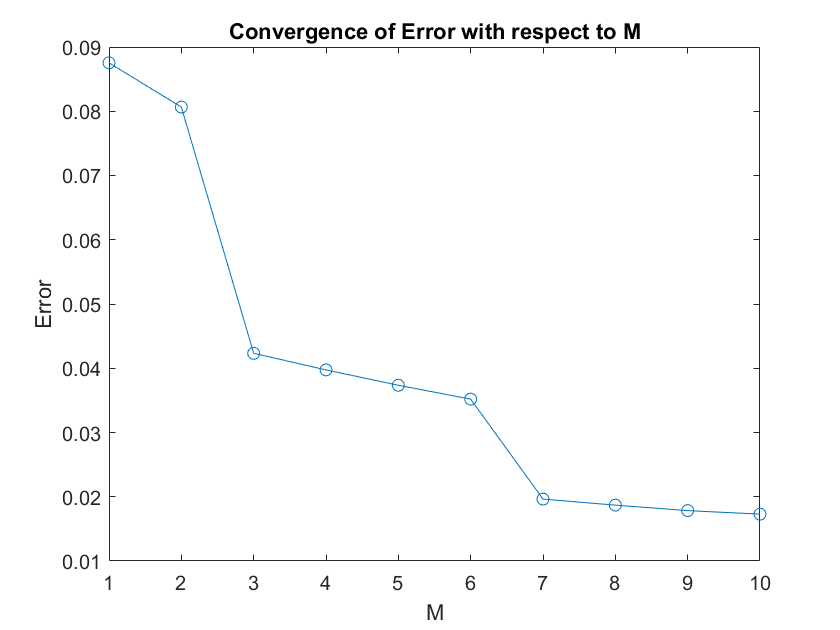
\includegraphics[width=0.6\textwidth]{pdes/fig/converge_error_m.png}
    \caption{Convergence of error with respect to $M$}
    \label{fig:converge_error_m}
\end{figure}

Figure \ref{fig:converge_error_m} shows the convergence of the error of the Finite Difference Method (FDM) solution as the number of time steps, $M$, increases.

\begin{figure}[H]
    \centering
    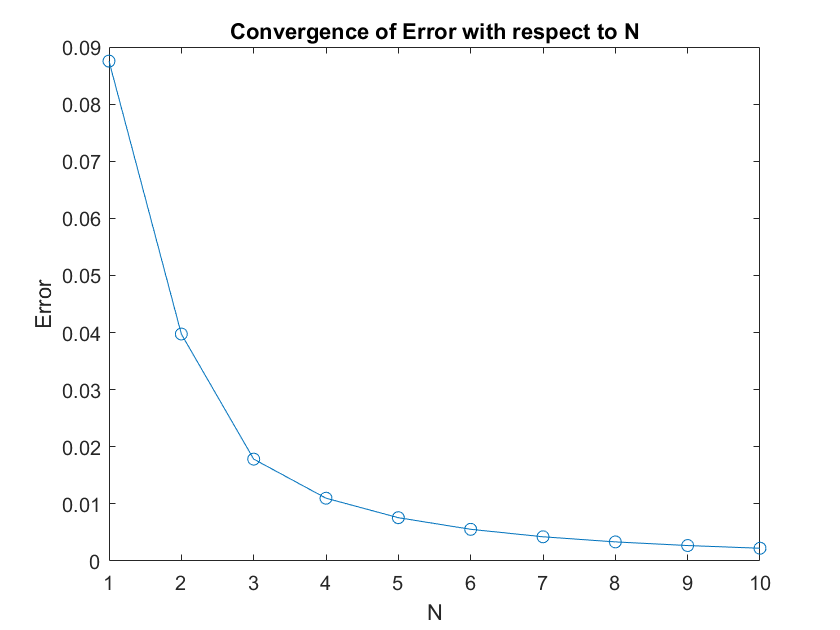
\includegraphics[width=0.6\textwidth]{pdes/fig/converge_error_n.png}
    \caption{Convergence of error with respect to $N$}
    \label{fig:converge_error_n}
\end{figure}

Figure \ref{fig:converge_error_n} illustrates the convergence of the error of the FDM solution as the number of spatial grid points, $N$, increases.

% Add MATLAB code reference
The MATLAB implementation used for generating the convergence error graphs can be found in Appendix \ref{app:convergence_of_heateq_fdm}. In addition, the code is provided in Listing \ref{lst:convergence_of_heateq_fdm} in the appendix.

\subsubsection{The Finite Element Method (FEM)}

The finite element method (FEM) is a numerical technique for solving partial differential equations (PDEs) by discretizing the domain into a collection of finite elements. The basic idea behind the FEM is to represent the solution within each element using a set of basis functions. These basis functions are typically chosen as continuous piecewise polynomials across the element boundaries. By expressing the solution as a linear combination of these basis functions, we can approximate the PDE within each element.

The variational formulation is a vital component of the finite element method. It involves transforming the PDE into an equivalent variational problem, where the goal is finding a solution that minimizes a specific function. This function is typically derived by multiplying the PDE with a test function and integrating it over the domain.

For example, let's consider the heat equation in one dimension:
\[
\partial_t u - \partial_{xx} u = f
\]
To obtain the variational formulation, we multiply the equation by a smooth test function \(v \in C^{\infty}_0(G)\) satisfying \(v(a) = v(b) = 0\), where \(G\) is the domain. 

Then, integrating the heat equation on the whole domain \(G\), we have:
\[
\int_G v \partial_t u\, dx - \int_G v \partial_{xx} u\, dx = \int_G vf\, dx
\]

Now, integrating by parts:
\[
\frac{{d}}{{dt}}\int_G u v \, dx - \left[\partial_x u (t, x) v(x) \right]_{x=a}^{x=b} + \int_G \partial_{x} u \partial_{x} v\, dx = \int_G f v\, dx
\]

Since $v$ is zero on boundaries, the second term on the left-hand side is cancelled (it equals zero).

This equation represents the variational or weak formulation of the heat equation. The goal of the finite element method is to find the solution \(u\) such that \(u(0, x) = u_0(x)\) and, for all smooth test functions \(v \in C^{\infty}_0(G)\), the following equation holds:
\[
\frac{{d}}{{dt}}\int_G u(t, x)v(x)\, dx + \int_G u'(t, x) v'(x)\, dx = \int_G f(t, x) v(x)\, dx
\]
